\documentclass[journal]{vgtc}                % final (journal style)
%\documentclass[review,journal]{vgtc}         % review (journal style)
%\documentclass[widereview]{vgtc}             % wide-spaced review
%\documentclass[preprint,journal]{vgtc}       % preprint (journal style)
%\documentclass[electronic,journal]{vgtc}     % electronic version, journal

%% Uncomment one of the lines above depending on where your paper is
%% in the conference process. ``review'' and ``widereview'' are for review
%% submission, ``preprint'' is for pre-publication, and the final version
%% doesn't use a specific qualifier. Further, ``electronic'' includes
%% hyperreferences for more convenient online viewing.

%% Please use one of the ``review'' options in combination with the
%% assigned online id (see below) ONLY if your paper uses a double blind
%% review process. Some conferences, like IEEE Vis and InfoVis, have NOT
%% in the past.

%% Please note that the use of figures other than the optional teaser is not permitted on the first page
%% of the journal version.  Figures should begin on the second page and be
%% in CMYK or Grey scale format, otherwise, colour shifting may occur
%% during the printing process.  Papers submitted with figures other than the optional teaser on the
%% first page will be refused.

%% These three lines bring in essential packages: ``mathptmx'' for Type 1
%% typefaces, ``graphicx'' for inclusion of EPS figures. and ``times''
%% for proper handling of the times font family.

\usepackage{mathptmx}
\usepackage{graphicx}
\usepackage{times}
\usepackage{subcaption}
\usepackage{multicol}

%% We encourage the use of mathptmx for consistent usage of times font
%% throughout the proceedings. However, if you encounter conflicts
%% with other math-related packages, you may want to disable it.

%% This turns references into clickable hyperlinks.
\usepackage[bookmarks,backref=true,linkcolor=black]{hyperref} %,colorlinks
\hypersetup{
  pdfauthor = {},
  pdftitle = {},
  pdfsubject = {},
  pdfkeywords = {},
  colorlinks=true,
  linkcolor= black,
  citecolor= black,
  pageanchor=true,
  urlcolor = black,
  plainpages = false,
  linktocpage
}

%% If you are submitting a paper to a conference for review with a double
%% blind reviewing process, please replace the value ``0'' below with your
%% OnlineID. Otherwise, you may safely leave it at ``0''.
\onlineid{0}

%% declare the category of your paper, only shown in review mode
\vgtccategory{Research}

%% allow for this line if you want the electronic option to work properly
\vgtcinsertpkg

%% In preprint mode you may define your own headline.
%\preprinttext{To appear in an IEEE VGTC sponsored conference.}

%% Paper title.

\title{Framework for comparing 3D Scatterplot Analysis in Immersive and Non-Immersive Environments using Smartphones}

%% This is how authors are specified in the journal style

%% indicate IEEE Member or Student Member in form indicated below
\author{Kartik Prabhu, Vikram Apilla, and Prof. Bernhard Preim}
\authorfooter{
%% insert punctuation at end of each item
\item Kartik Prabhu, MSc. in Digital Engineering student\textsuperscript{1}. 
\newline E-mail: kartik.prabhu@st.ovgu.de.
\item Vikram Apilla, MSc. in Data and Knowledge Engineering student\textsuperscript{1}.  
\newline E-mail: vikram.apilla@st.ovgu.de.
\item Bernhard Preim, Professor and Head of the Visualization group\textsuperscript{1}.  \newline E-mail: bernhard.preim@ovgu.de.
\vspace{0.1cm}
\newline \textsuperscript{1}Otto-von-Guericke-Universität Magdeburg
}

%other entries to be set up for journal
\shortauthortitle{Biv \MakeLowercase{\textit{et al.}}: Global Illumination for Fun and Profit}
%\shortauthortitle{Firstauthor \MakeLowercase{\textit{et al.}}: Paper Title}

%% Abstract section.
\abstract{The report is a description of the project in which we propose a framework to make a comparison of user performance in data visualization using a smartphone. The data visualization technique and the evaluation method considered here is a 3D scatterplot and a controlled user study respectively. The user study proposed is based on the scatterplot analysis, with tasks consisting of namely \textit{Outlier Detection}, \textit{Cluster Analysis}, and \textit{Correlation Detection}. These tasks would be performed in different environments and on different datasets varying in terms of the size of points as shown in Fig. 1 as a sample. For example, a task, based on \textit{Outlier Detection} would be performed on different datasets, and in different environments(immersive and non-immersive). Further, the framework also includes a few hypotheses and ways to assess them. Based on the results recorded from the user study, one could make a comparison between user performances over different datasets between immersive and non-immersive environments. With the help of this project's framework, conclusions could be drawn about the strengths and limitations of data visualisation using a smartphone.
} % end of abstract

%% Keywords that describe your work. Will show as 'Index Terms' in journal
%% please capitalize first letter and insert punctuation after last keyword
\keywords{3D Scatterplots, Augmented Reality, Immersive Analytics, User Study}

%% ACM Computing Classification System (CCS). 
%% See <http://www.acm.org/class/1998/> for details.
%% The ``\CCScat'' command takes four arguments.

% \CCScatlist{ % not used in journal version
%  \CCScat{K.6.1}{Management of Computing and Information Systems}%
% {Project and People Management}{Life Cycle};
%  \CCScat{K.7.m}{The Computing Profession}{Miscellaneous}{Ethics}
% }

%% Uncomment below to include a teaser figure.
\teaser{
     \centering
     \begin{subfigure}[t]{0.225\textwidth}
        \centering
        \includegraphics[width=4cm]{img/0_a.PNG}
        \caption{}
     \end{subfigure}%
    ~ 
     \begin{subfigure}[t]{0.225\textwidth}
        \centering
        \includegraphics[width=4cm]{img/0_b.PNG}
        \caption{}
     \end{subfigure}%
    ~ 
     \begin{subfigure}[t]{0.225\textwidth}
        \centering
        \includegraphics[width=4cm]{img/0_c.PNG}
        \caption{}
     \end{subfigure}%
    ~ 
     \begin{subfigure}[t]{0.225\textwidth}
        \centering
        \includegraphics[width=4cm]{img/0_d.PNG}
        \caption{}
     \end{subfigure}%
    \caption{Different Datasets: from left to right, the number of data points in the 3D scatterplots are in increasing order.}
  }

%% Uncomment below to disable the manuscript note
\renewcommand{\manuscriptnotetxt}{}

%% Copyright space is enabled by default as required by guidelines.
%% It is disabled by the 'review' option or via the following command:
% \nocopyrightspace

%%%%%%%%%%%%%%%%%%%%%%%%%%%%%%%%%%%%%%%%%%%%%%%%%%%%%%%%%%%%%%%%
%%%%%%%%%%%%%%%%%%%%%% START OF THE PAPER %%%%%%%%%%%%%%%%%%%%%%
%%%%%%%%%%%%%%%%%%%%%%%%%%%%%%%%%%%%%%%%%%%%%%%%%%%%%%%%%%%%%%%%%

\begin{document}

%% The ``\maketitle'' command must be the first command after the
%% ``\begin{document}'' command. It prepares and prints the title block.

%% the only exception to this rule is the \firstsection command
\firstsection{Introduction}

\maketitle
%% \section{Introduction} %for journal use above \firstsection{..} instead
We live in an age of data where every aspect of our lives is digitally recorded. With the increasing amount of data, the technologies to visualize it has also been growing at a rapid rate. One could be interested in using the latest technologies to visualize the data to understand the information, patterns and dependencies from it. These technologies include devices such as \textit{VR Glasses} and \textit{HoloLens} which helps in immersive data visualization, but, the caveat here is that they are not always at the reach of a user. One device which has been around for a while and also the one that is frequently accessed on-demand by a user is a mobile phone. Mobile phones have evolved incredibly over the past decade that they are now called \textit{Smartphones}. The idea of this project is to exploit the features provided by the current generation of smartphones in visualizing the data, specifically 3D scatterplots.

Every year, we are witnessing a massive growth in terms of computational power and features that are available through smartphones. Although they are small, these devices are used by almost everyone because of their compactness and functionalities. Every industry, right from entertainment to education, is targeting a smartphone as one of the major platforms. The device offers extensive capabilities such as video streaming, online gaming, and even acting as a virtual assistant. Tech giants, in particular, Google and Apple have invested their time on building augmented reality Software-Development-Kits so that new immersive applications can be developed on mobile platforms with ease. With all these advances and developments in a personal device, one could think, if it is possible to visualize 3D data immersively with the current generation of smartphones with high-resolution displays, and their ability to provide augmented reality features.

\begin{figure}[ht]
    \begin{minipage}[b]{0.45\linewidth}
        \centering
        \includegraphics[width=\textwidth]{img/01_outlier_detection.PNG}
        \subcaption{Outlier Detection}
    \end{minipage}
    \hspace{0.5cm}
    \begin{minipage}[b]{0.45\linewidth}
        \centering
        \includegraphics[width=\textwidth]{img/04_correlation.PNG}
       \subcaption{Correlation Detection}
    \end{minipage}
    \caption{Detecting tasks presented to the user}
\end{figure}

In this project, our focus is on the comparisons made based on user performances in scatterplot analysis using a smartphone supported with augmented reality. With that under consideration, the project can be divided into two parts. The first part helps in addressing, how smartphones could be useful in visualizing different datasets varying in terms of their size. The second part helps in understanding the immersiveness with which a user can visualize the data in augmented reality setup using the smartphone as compared to a non-augmented reality. Considering both of them, it would be interesting to answer the research question \textit{How effective is 3D scatterplots visualization of different datasets in different environments(immersive and non-immersive) using a smartphone?}\cite{cliquet2017towards}\cite{lu2016towards}

The report is further organized into different sections. Firstly, the \textit{Background} section gives a broad overview of the major components involved in the project.  Secondly, a summary of closely related published papers is discussed in the \textit{Related Work} to understand prior research. This is then followed by the proposed \textit{Hypotheses} of the project. Then, a detailed description of how the controlled user study could be conducted using the framework is given in the \textit{Study Design} section. Furthermore, a short text about the \textit{Evaluation} is made to understand what could be expected of the framework once the user study is completed. Finally, final remarks of the project are provided in the \textit{Discussion} and \textit{Conclusions and Future Work} sections.


\begin{figure}[ht]
    \begin{minipage}[b]{0.45\linewidth}
        \centering
        \includegraphics[width=\textwidth]{img/02_cluster_estimation.PNG}
        \subcaption{Clusters Estimation}
    \end{minipage}
    \hspace{0.5cm}
    \begin{minipage}[b]{0.45\linewidth}
        \centering
        \includegraphics[width=\textwidth]{img/03_cluster_assignment.PNG}
        \subcaption{Cluster Assignment}
    \end{minipage}
    \caption{Estimating tasks presented to the user}
\end{figure}

\section{Background}

In this section, we briefly describe the important facets of this project. The purpose is to provide the user with enough knowledge to understand further topics better.

\subsection{Augmented Reality}

Augmented reality is "An interactive combination of reality and virtuality"\cite{Billinghurst2014}. The rendering is performed in real-time and 3D objects are registered (geometrically). One can view the world around them through their smartphone cameras while projecting an augmented object as overlays, that makes it seem as if the virtual objects were real. The applications in the field of augmented reality are tremendous. One of the most trending games of all time, Pokemon Go, is based on augmented reality, which made the world of Pokemon come to life. Through this, the users got the immersive experience of the gaming world. Similarly, in this project, we will conduct a study of how augmented reality gives an immersive experience with data visualisation to the users.
 
 
\subsection{Immersive Analytics}
Understanding the data and making decisions based on it using the latest technologies such as \textit{Large Displays, Augmented Reality}, and \textit{Virtual Reality} is called as \textit{Immersive Analytics} \cite{Chandler2015}\cite{bach2016immersive}. Scenarios including egocentric methods such as data visualization using virtual reality, or multi-user visual analytics using large displays are all good examples of Immersive Analytics. A considerable amount of research is being carried out in this new area of data analytics. In this project, we would like to conduct our part of the research by focusing extensively on the immersive environment Augmented Reality with the help of a smartphone.

\subsection{Scatterplots}
A scatterplot is a type of plot or mathematical diagram used to represent distributions of 2 or more continuous variables of a dataset. It helps to understand associations between variables and to understand the sparsity of the dataset. Analysis of clusters, correlations and identification of outliers are some of the typical uses of scatterplots \cite{Tufte1983}.

\section{Related Work}

There has been prior research conducted in mobile phone data visualization and augmented reality-based 3D visualizations. In the following, we summarize three closely related research to our work.

In 2006, Buering et al. \cite{buering2006user} published their work about data visualization of 7500 data points in a scatterplot using a mobile phone. In their work, they made a comparison between two different zooming techniques, Geometric-Semantic Zoom and Fisheye Distortion. While the results between these techniques were indistinguishable, it was interesting to see that there was research conducted in mobile data visualization back in the years where smartphones were not as powerful as they are now.

Butcher et al. \cite{butcher2016immersive} have proposed a cost-effective solution for Immersive Analytics in 2016. In their work, they have successfully made use of the economical Google Cardboard coupled with a smartphone for data visualization using virtual reality. Although they have effectively built an immersive environment, it has to be noted that to take actions such as highlighting and zooming without the hand controllers proved to be difficult. In this project, we try to avoid this by switching the environment to augmented reality and thereby providing the user with complete control to take action using their phone through natural gestures.

Recently, another research which is closely related to this project was published in the year 2017 by Bach et al. \cite{bach2017hologram}. Their work consisted of a user study based on the comparison of 3D visualizations between three different environments - Desktop, HoloLens and a Tablet. While their results showed that desktop was faster in terms of task completion, HoloLens led the way in immersion.

All of these prior research has laid a good foundation for further research to be conducted in the area of Immersive Analytics, mainly in this case, using a smartphone.

\begin{figure}[ht]
    \begin{minipage}[b]{0.45\linewidth}
        \centering
        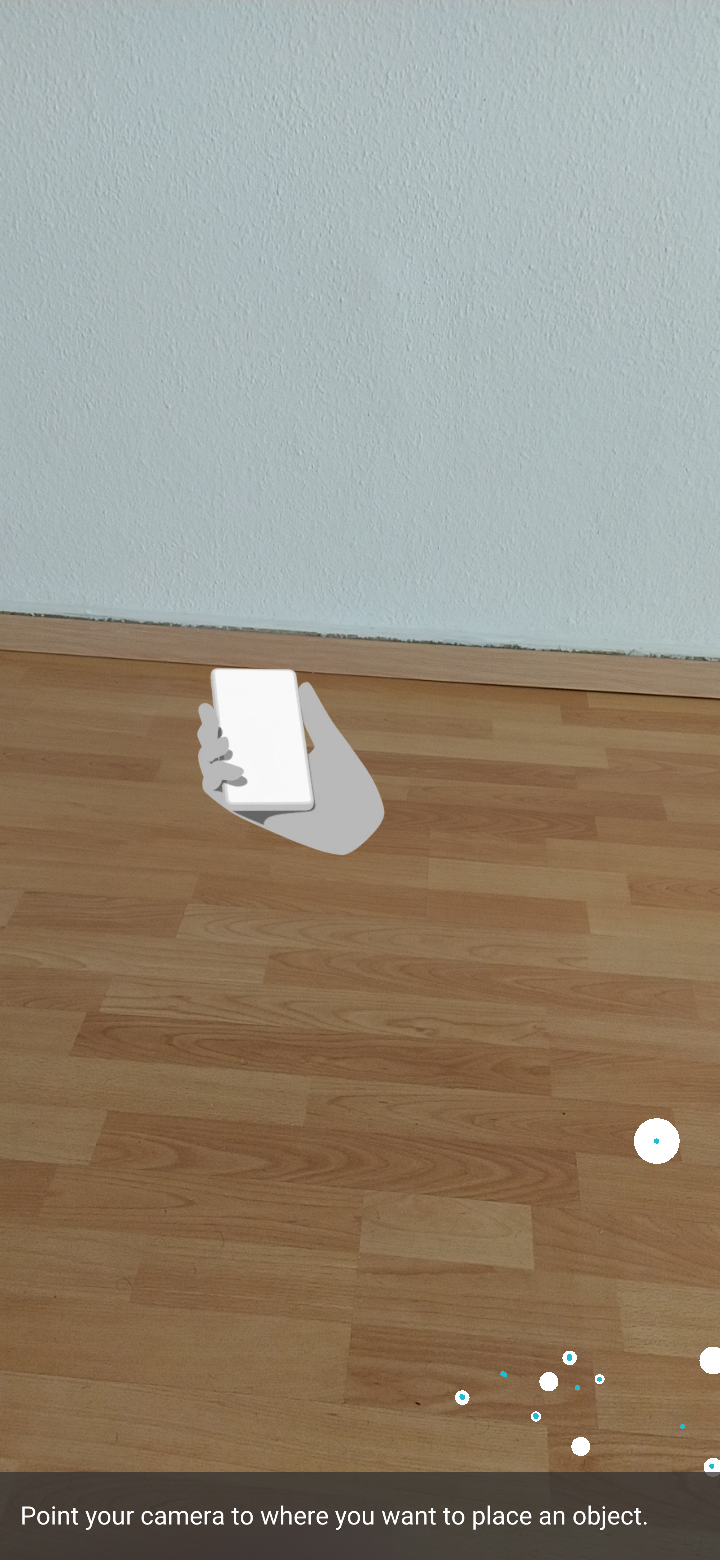
\includegraphics[width=\textwidth, height=2.5in]{animation.png}
        \subcaption{}
    \end{minipage}
    \hspace{0.5cm}
    \begin{minipage}[b]{0.45\linewidth}
        \centering
        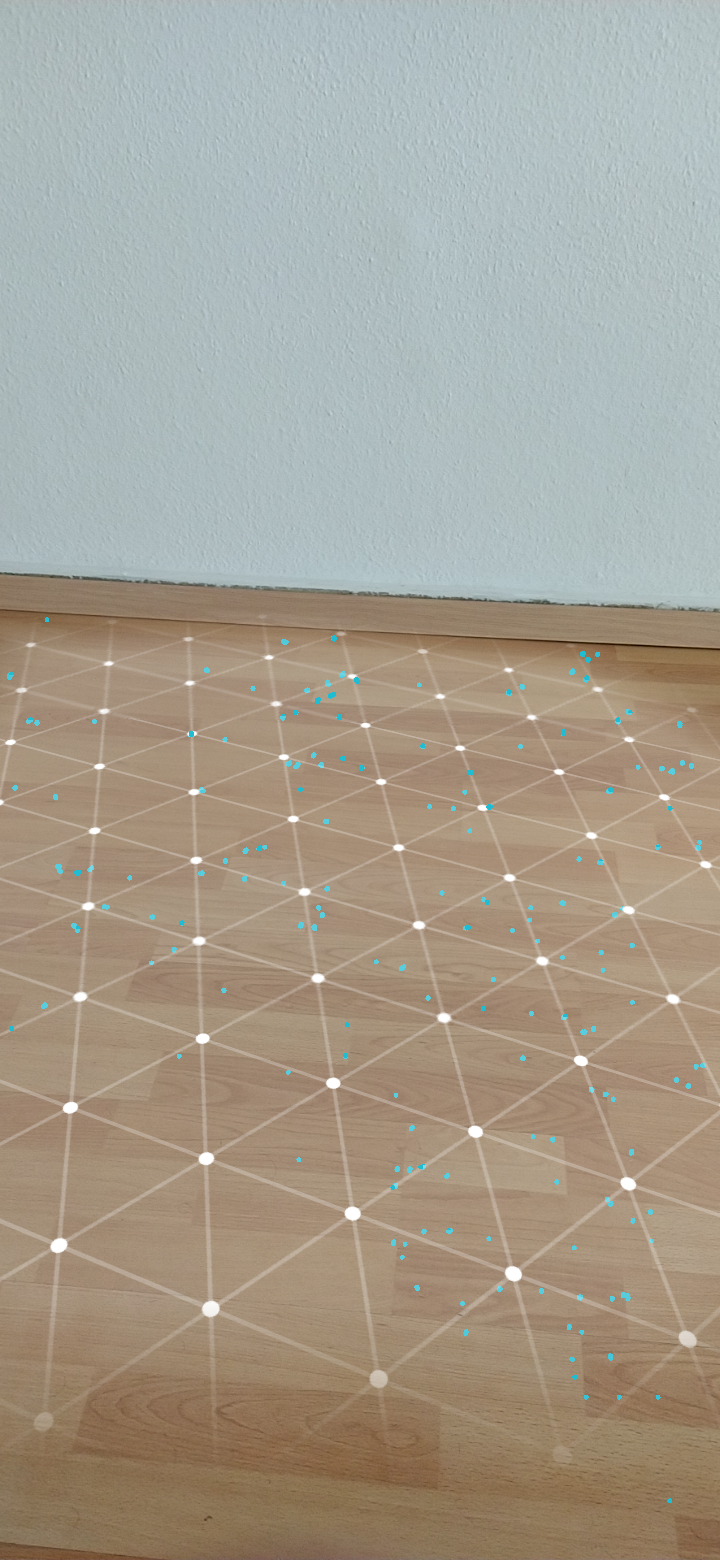
\includegraphics[width=\textwidth, height=2.5in]{planedetection.png}
       \subcaption{}
    \end{minipage}
    \caption{(a) Animation to help user detect plane (b) Detected horizontal plane to register the plot object}
\end{figure}

\begin{figure*}
\begin{multicols}{5}
    \begin{minipage}[b]{\linewidth}
    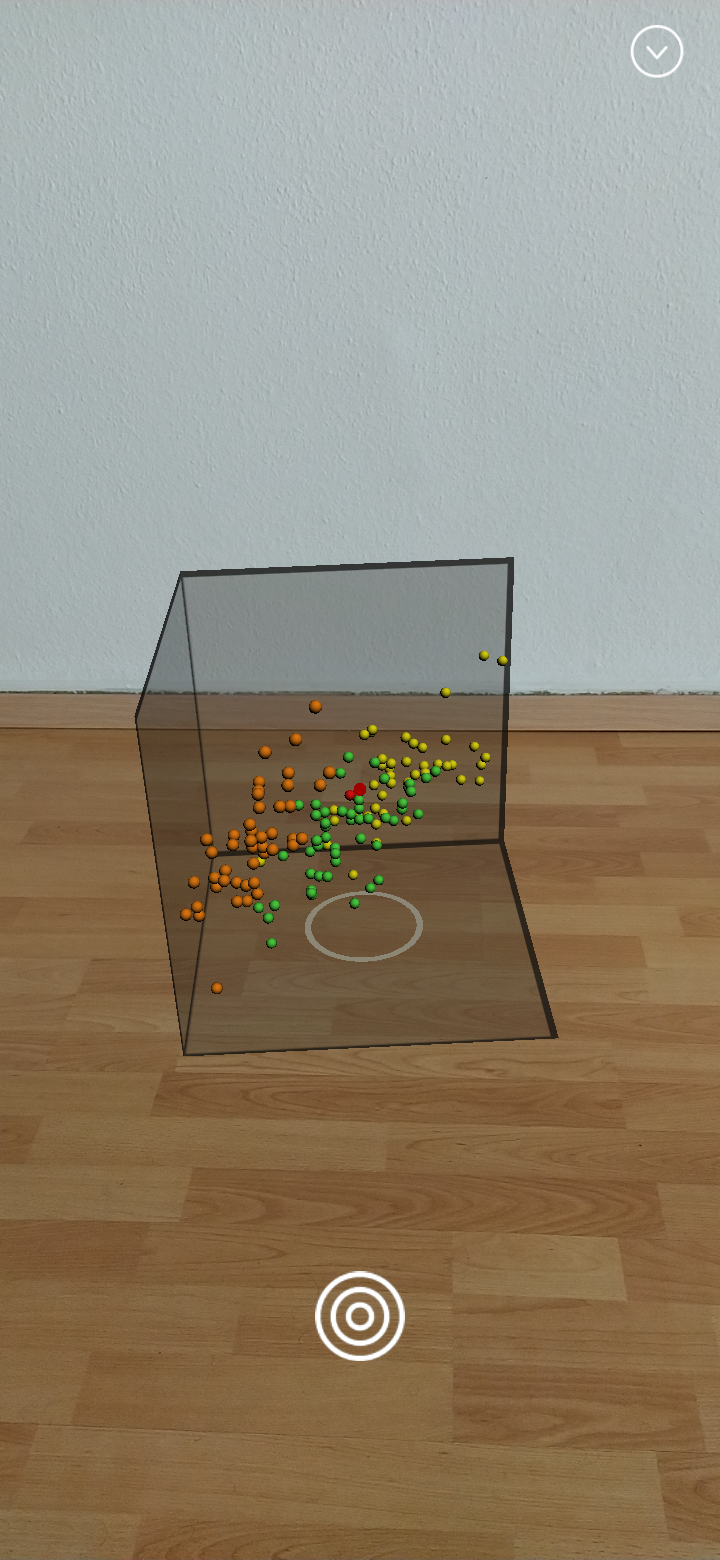
\includegraphics[width=\linewidth]{initial.png}\par 
    \subcaption{Initial position}
    \end{minipage}
    
    \begin{minipage}[b]{\linewidth}
    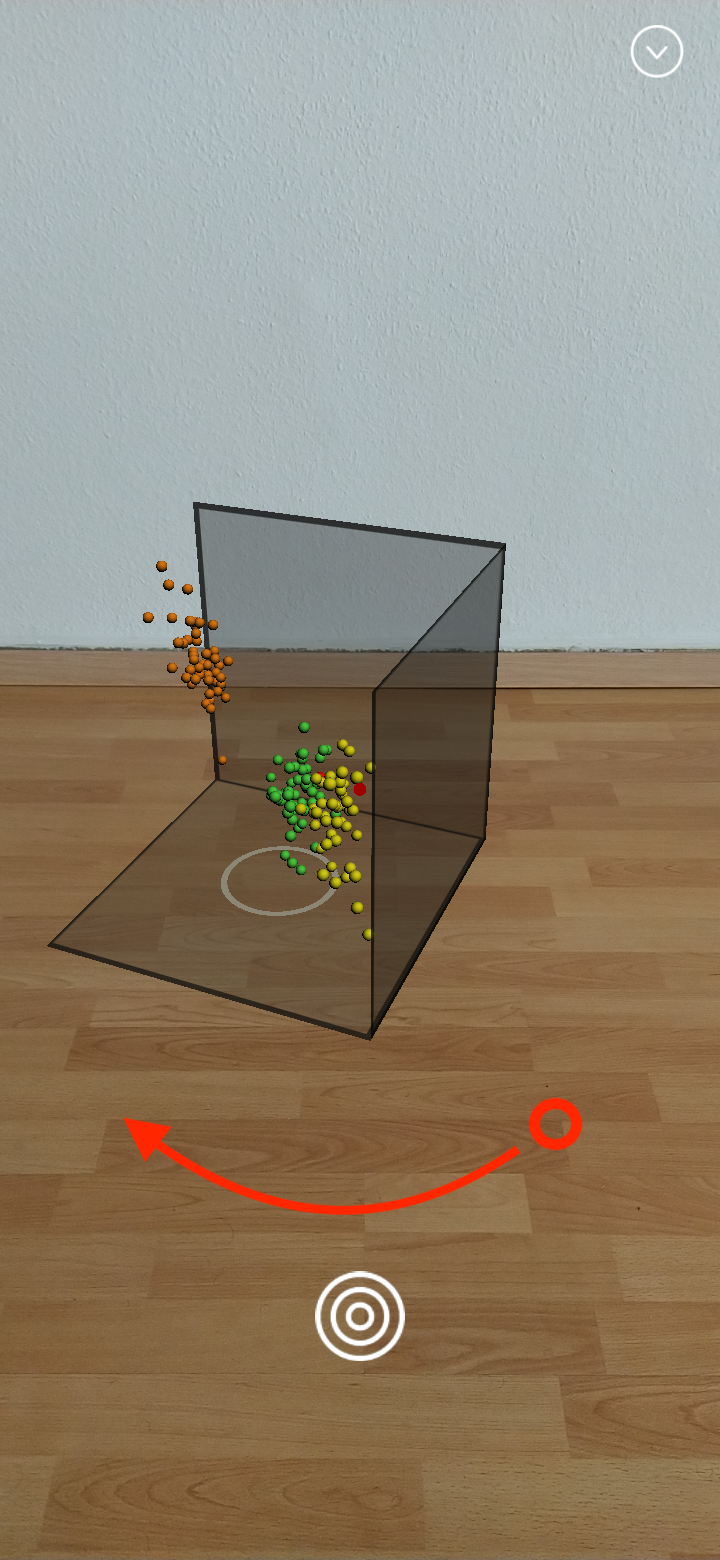
\includegraphics[width=\linewidth]{rotation.png}\par 
    \subcaption{Rotation}
    \end{minipage}
    
    \begin{minipage}[b]{\linewidth}
    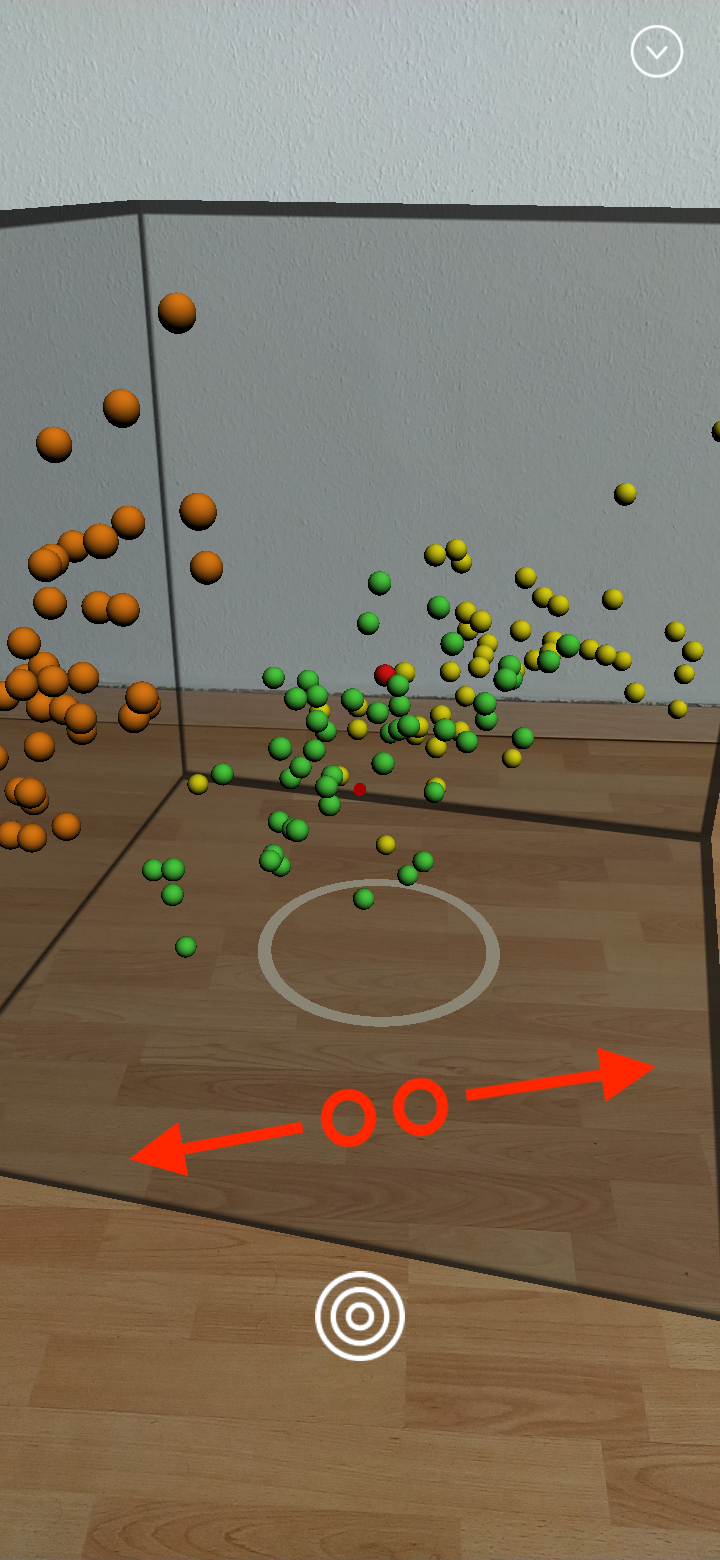
\includegraphics[width=\linewidth]{zoom.png}\par
    \subcaption{Zoom}
    \end{minipage}
        
    \begin{minipage}[b]{\linewidth}
    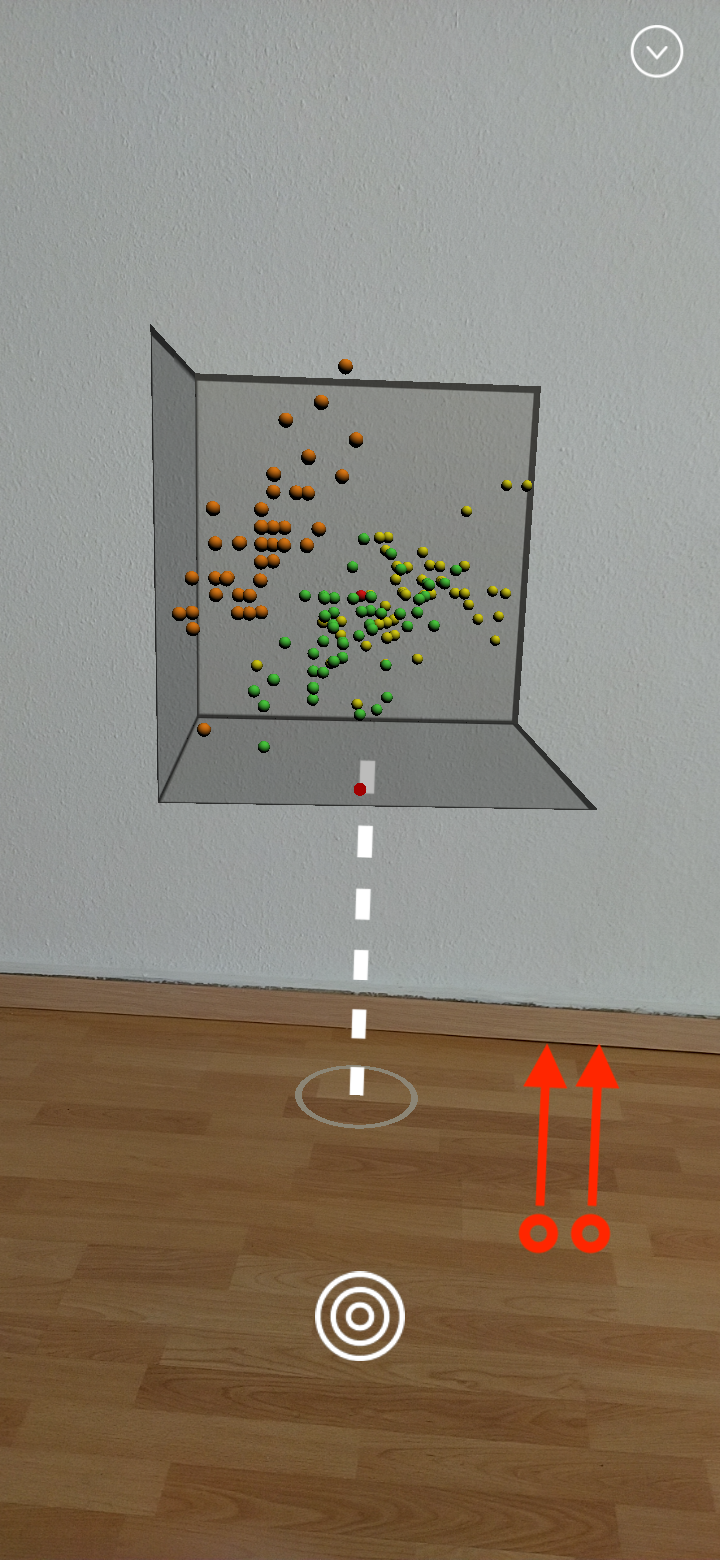
\includegraphics[width=\linewidth]{elevation.png}\par
    \subcaption{Elevation}
    \end{minipage}
        \begin{minipage}[b]{\linewidth}
    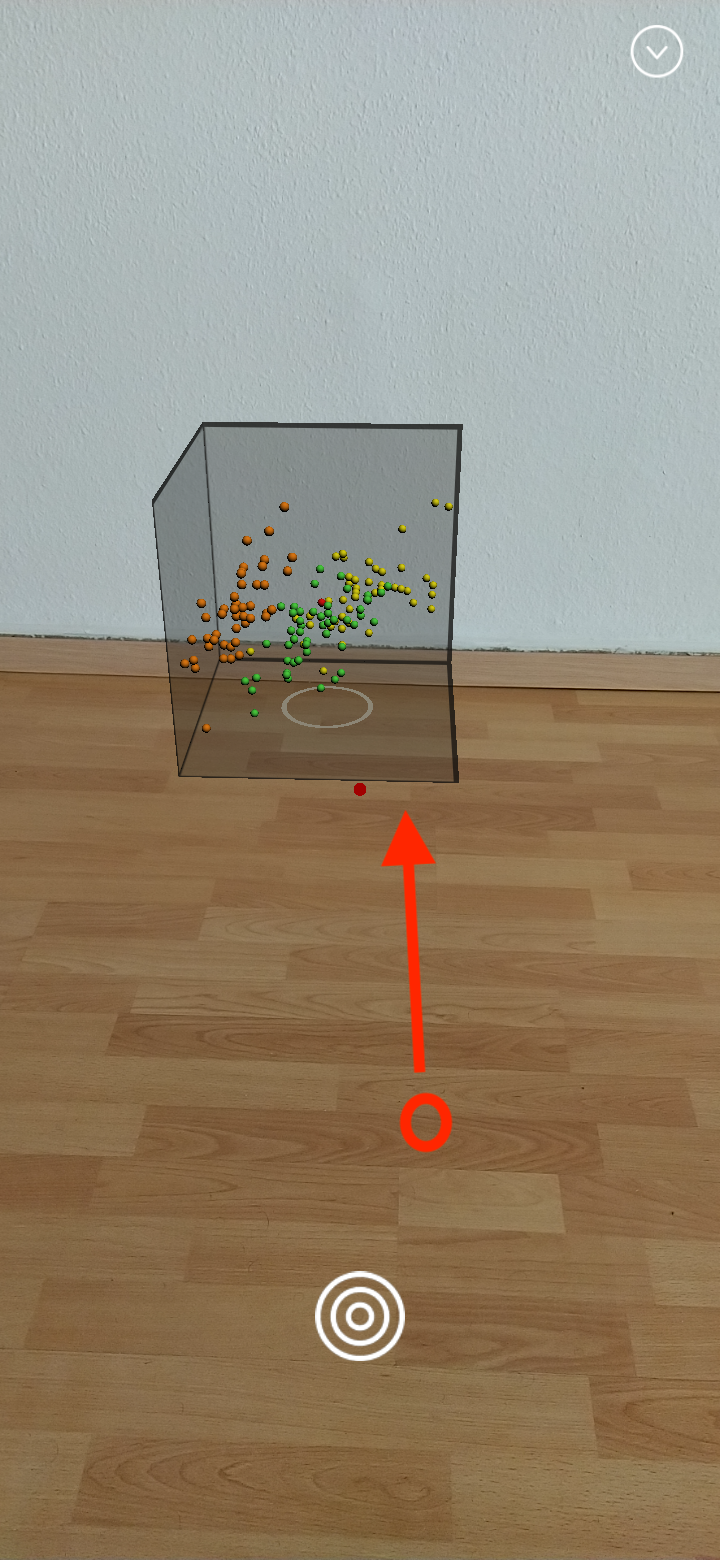
\includegraphics[width=\linewidth]{transition.png}\par
    \subcaption{Translation}
    \end{minipage}
\end{multicols}
\caption{Multi-touch gesture support using ARcore manipulation system. A tap and drag outside the object rotates, pinch for zoom, 2 finger tap and vertical drag for elevation, tap on object and drag for translation (left to right).}
\end{figure*}

\section{Implementation}

The application for scatterplot analysis was built on the Android platform with the support of ARCore library on Unity3D. ARCore enables a supported smartphone to sense and interact with the environment around it. It is based on 3 key features - motion tracking, environmental understanding and light estimation. The library makes use of sensors (accelerometer, gyroscope, light sensor) present in the smartphones to enable these features.

ARCore also supports a manipulation system. User can  \textit{Scale} the entire plot uniformly in all directions with a pinch gesture. \textit{Rotation} and \textit{Translation} interactions are similar as described by Kruger et. al\cite{Kruger2005}. A central circular area (~25\% of the object size) is defined where the object is translated. With a contact point outside, a movement with a pointing device or touch rotates the object. Using 2 fingers perpendicular motion, user can elevate the plot. All these manipulations have only one degree of freedom.

The augmented plot object can be placed on a detected plane. Plot placement follows the general guideline that the object should move along a supporting surface or an artificial interaction plane, in this case, the detected plane surface. The plot placement supports two interaction task as mentioned in \cite{Teather2007}: a new object is inserted in the virtual environment and an existing object is selected, picked up and placed elsewhere, but the 3rd task of translating incrementally is not supported, as mobile devices don’t have explicit keys. An animation to guide the user on how to detect a plane is also implemented.

For the selection of glyph points in the scatterplots, raycasting is implemented within the application. Considering the large number of data points that would be used in the user study, spatial cues such as shadows, grid lines, and ghost cuts would not be helpful as shown by the research from Luboschik et al. \cite{luboschik2016spatial}. Hence, they are not included in the framework application. Rather, to assist the user, the co-ordinates and point number is displayed in a tooltip which appears above the plot while always looking at the camera as shown in Fig.

In the case of non-augmented reality environment, for selection of glyphs, a cross-hair selector controlled by a joystick on screen is implemented as illustrated in Fig. Manipulation system consists of scaling and rotation with y-axis as the pivot. Tooltip support, just like in the augmented reality environment is given.  

\begin{figure}[ht]
    \begin{minipage}[b]{0.45\linewidth}
        \centering
        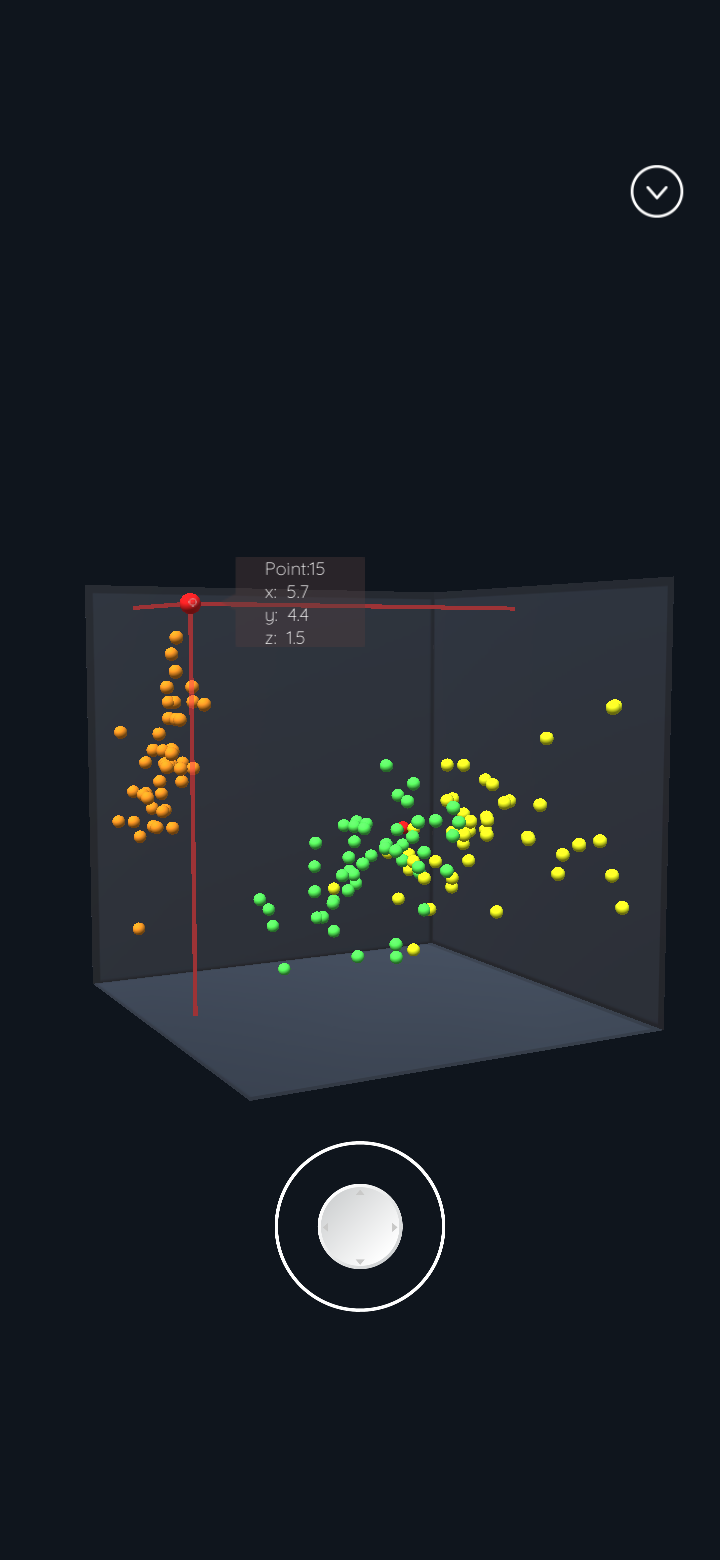
\includegraphics[width=\textwidth, height=2.5in]{img/non_ar_tooltip_crosshair.png}
        \subcaption{Non-AR tooltip with joystick}
    \end{minipage}
    \hspace{0.5cm}
    \begin{minipage}[b]{0.45\linewidth}
        \centering
        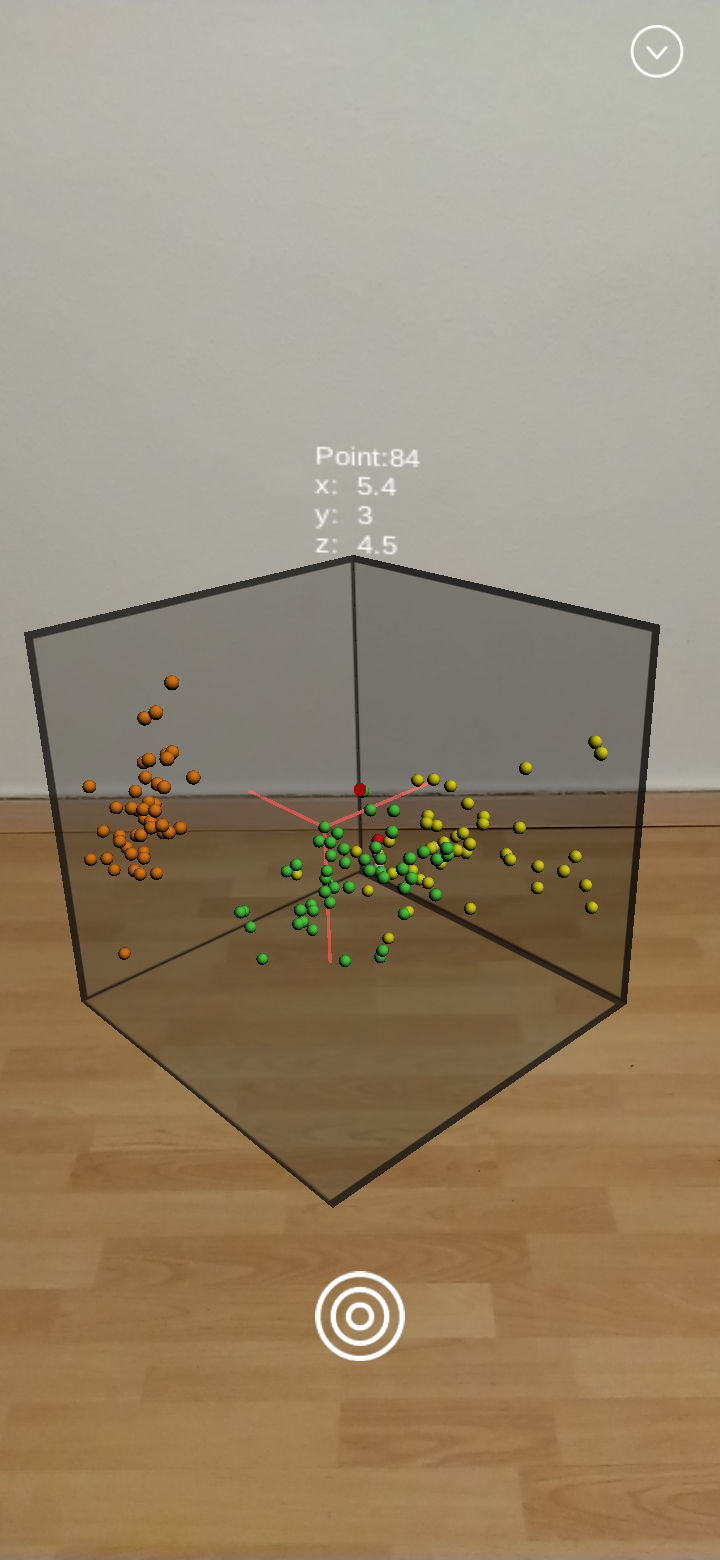
\includegraphics[width=\textwidth, height=2.5in]{img/ar_tooltip.png}
       \subcaption{AR tooltip with raycast selector}
    \end{minipage}
    \caption{Selectors and tooltips in different environments}
\end{figure}


\section{Study Design}
This section covers the details about the controlled user study to evaluate the user performance \cite{lam2011empirical}.
\subsection{Device}
The device used for the study is Xiaomi Mi A3, supported on Android-one program, running on Android 9 OS. It meets the minimum SDK version of 27 to support ARCore library(1.15.0). The device consists of Qualcomm\textsuperscript{\textregistered} Snapdragon™ 665 processor with a Super AMOLED Display of 15.46cm (6.08) and HD+ display (1560 x 720). The advantage of having a smartphone in the experiment is that the user can use regular gestures for manipulating the object in the screen.


\subsection{Environments}
As the tasks would be based on the comparison between augmented reality-based and non-augmented reality-based scatterplots, the application used for the study would contain both the environments.
\subsubsection{\textit{With Augmented Reality}}
With augmented reality, the user would be able to register the plot in their desired location and use the phone's ability of the movement to analyse the plot.

\begin{figure}[ht]
    \begin{minipage}[b]{0.45\linewidth}
        \centering
        \includegraphics[width=\textwidth, height=2.5in]{ar.png}
        \subcaption{Augmented Reality}
    \end{minipage}
    \hspace{0.5cm}
    \begin{minipage}[b]{0.45\linewidth}
        \centering
        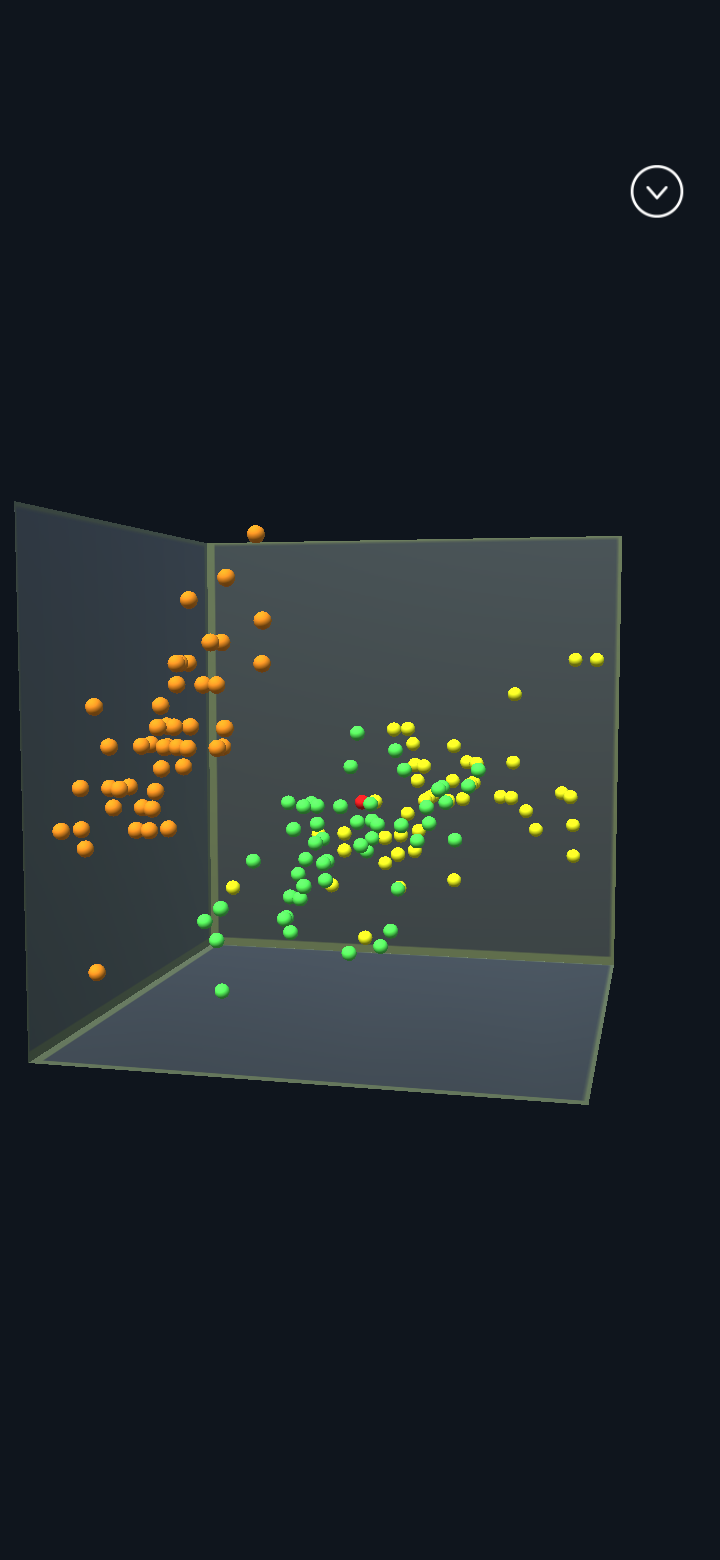
\includegraphics[width=\textwidth, height=2.5in]{non_ar.PNG}
       \subcaption{Non-Augmented Reality}
    \end{minipage}
    \caption{Different environments for user study}
\end{figure}

\subsubsection{\textit{Without Augmented Reality}}
In the case of the non-augmented environment, the plot would be displayed with a fixed background. While the provision of using simple finger gestures for manipulating the plots is provided, other features of the smartphone such as the camera, gyroscope and accelerometer are disabled. Thus, the user can only analyse the plot with limited movement like any other non-augmented reality application.

\subsection{Procedure}

The application for the survey is built in a quiz format, with the users able to record their responses either through a numerical or a multiple-choice. The task would not proceed unless the user submitted the answer for the ongoing task. The participants(users) would be split into two groups. One group allowed to perform the tasks with augmented reality, and the other without augmented reality. The reason for different groups is to introduce counterbalancing and avoid any confounding factors resulting from the user studies. Also, before the user study, every participant could be given a short tutorial on how to complete the user study.

The participants' tasks and responses are both presented and recorded respectively using an android application. The application would contain two different branches. One without augmented reality, and the other with augmented reality as shown in Fig. 4.

Along with the response to a task from the participants, the time taken to complete the task is also recorded automatically using the application. The time taken variable will help in comparing which environment had quicker responses compared to the other. It would be the basis for the qualitative and summative evaluation\cite{Lewis}. During the task, the number of interactions using different manipulation techniques is also observed. Only the immersion level will be based on users personal experience with the two given environments and will be noted with the Likert scale. 

\begin{table}
\begin{center}
\def\arraystretch{1.25}% 
\begin{tabular}{ |l|l|l| } 
 \hline
 \textbf{Dataset Name} & \textbf{Task} & \textbf{Data Points} \\ 
 \hline
 \hline
 Haberman’s Survival & Outlier Detection & 307 \\ 
 \hline
 Unknown & Outlier Detection & 700 \\ 
 \hline
 Iris & Cluster Assignment & 151 \\ 
 \hline 
 Seeds & Cluster Assignment & 211 \\ 
 \hline
 BigCity & Correlation Estimation & 50 \\ 
 \hline
 Unknow & Correlation Estimation & 99 \\ 
 \hline
 Letter & Performance Test & 20000 \\ 
 \hline
%  DS8 & Outlier Detection & 1000 \\ 
%  \hline
%  DS9 & Outlier Detection & 1000 \\ 
%  \hline
\end{tabular}
\caption{Table to test captions and labels}
\label{table:1}
\end{center}
\end{table}


\subsection{Datasets}

The datasets used for the user study is listed  in the table \ref{table:1} with its name, and the task it is used for and the number of points it contains.


\subsection{Tasks}

Three tasks are presented to the participants in the user study. The tasks are based on scatterplot analysis namely \textit{Outlier Detection}, \textit{Cluster Analysis}, and \textit{Correlation Detection}. Each task is presented thrice to the participant, every time the number of data points in the plot would vary. For example, consider \textit{Outlier Detection}, a participant would be asked to detect outliers in three different scatterplots, each plot with an increasing number of data points.

\subsubsection{Ground Truth for the tasks}

\subsubsection{\textit{Outlier Detection}}
A 3D scatterplot is presented to the user as shown in Fig.2 (a). Based on this scatterplot, the user would be asked for two responses. One is the number of outliers contained in the scatterplot. The other one is that which of the data points are part of the outliers. The latter response helps in understanding if the user has detected the right data points that are marked as outliers. 

\begin{figure}[ht]
    \begin{minipage}[b]{0.45\linewidth}
        \centering
        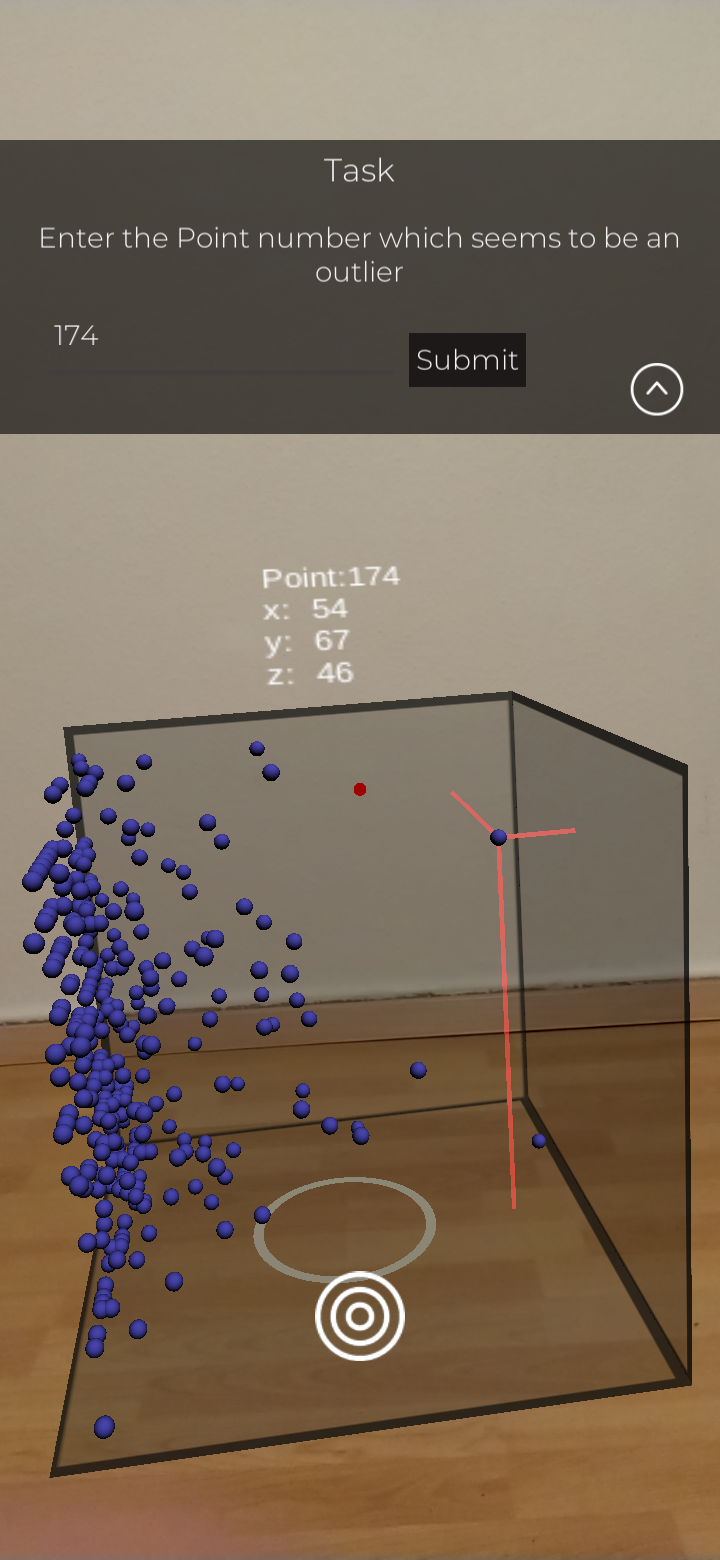
\includegraphics[width=\textwidth, height=2.5in]{Outlierdetection_task.png}
        \subcaption{Outlier detection task}
    \end{minipage}
    \hspace{0.5cm}
    \begin{minipage}[b]{0.45\linewidth}
        \centering
        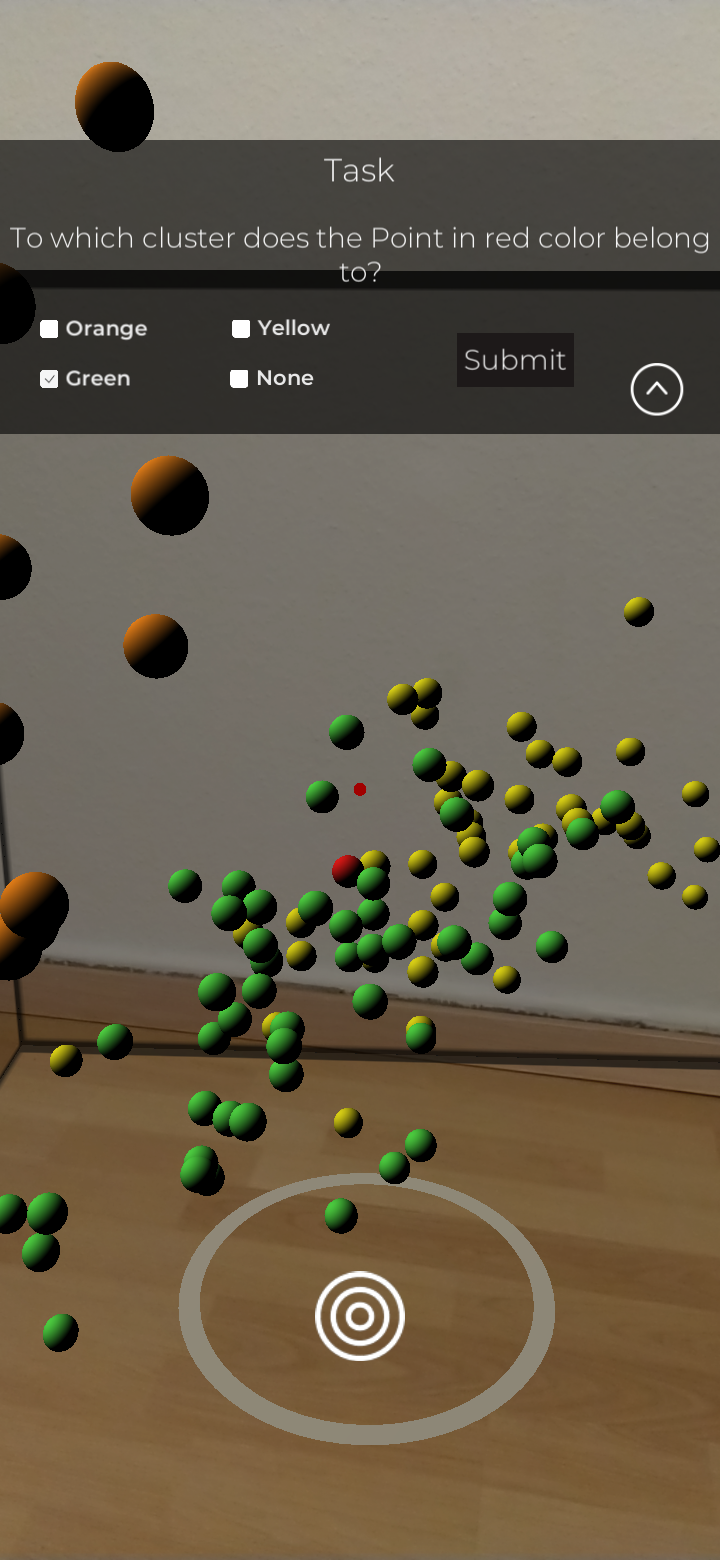
\includegraphics[width=\textwidth, height=2.5in]{clusterassignment_task.png}
       \subcaption{Cluster assignment}
    \end{minipage}
    \caption{Tasks in the survey. (a) Is an input type question where user has to type the answer (b) Is an multiple choice question.}
\end{figure}

\subsubsection{\textit{Cluster Analysis}}
The cluster analysis task is composed of two different sub-tasks as shown in Fig. 3.
\begin{enumerate}
    \item[i] \textit{Clusters Estimation}: a point cloud without colour is presented to the user. Based on this point cloud, the user has to estimate the total number of clusters present in the dataset. 
    \item[ii] \textit{Cluster Assignment}: the user has to assign a highlighted point in the point cloud to an appropriate cluster. For example, in Fig. 3 (b), the points that are enlarged and highlighted with magenta colour has to be assigned to one of the three clusters in green, white, or red. 
\end{enumerate}

\subsubsection{\textit{Correlation Detection}}
For the correlation detection, the user has to respond whether the scatterplot that is being presented has a strong correlation, weak correlation, positive correlation or negative correlation, linear, non-linear or planar. A sample of the correlation detection task can be found in Fig. 1 (d) and Fig. 2 (b). In both of these figures, the datasets contain a strong positive correlation.

\begin{figure}[ht]
    \begin{minipage}[b]{0.45\linewidth}
        \centering
        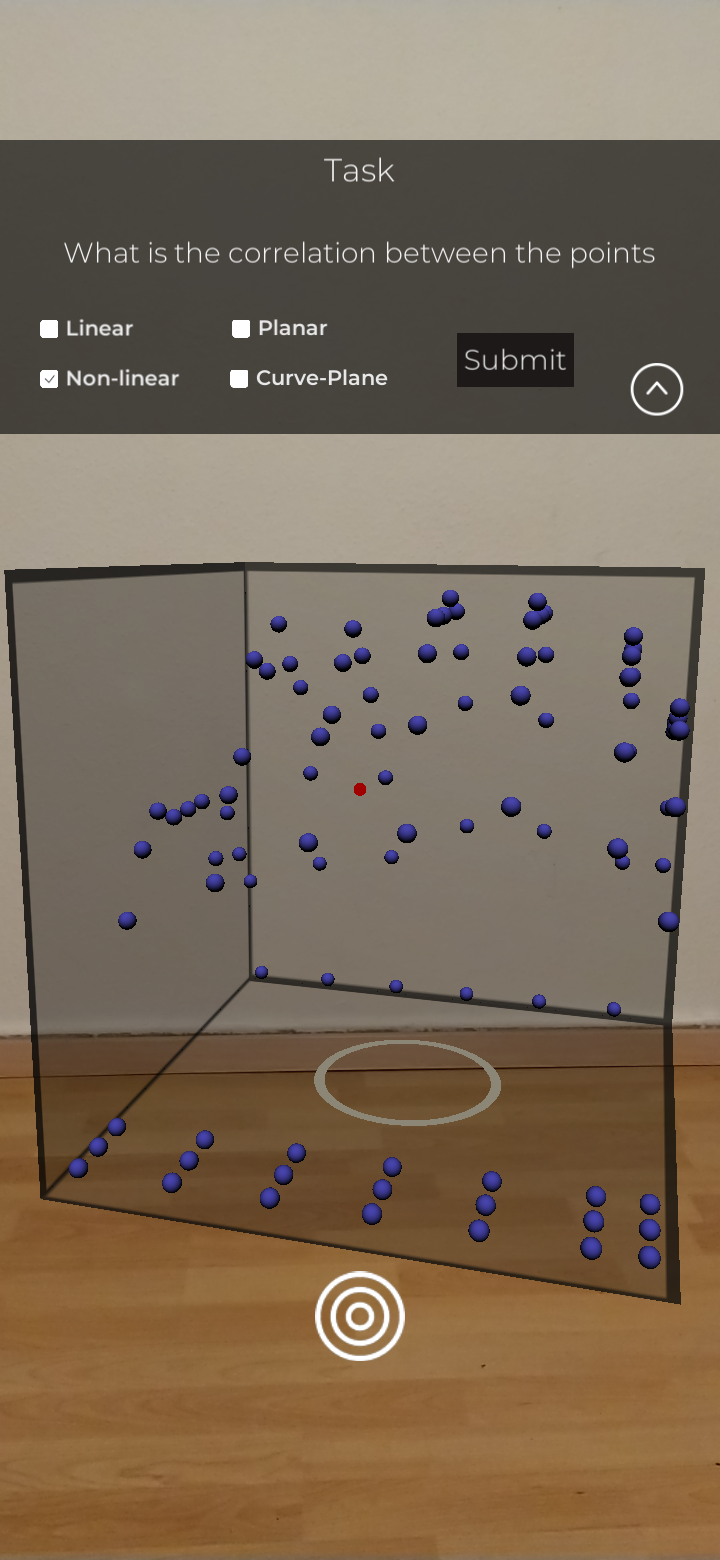
\includegraphics[width=\textwidth, height=2.5in]{correlation_frontview.png}
        \subcaption{Front view}
    \end{minipage}
    \hspace{0.5cm}
    \begin{minipage}[b]{0.45\linewidth}
        \centering
        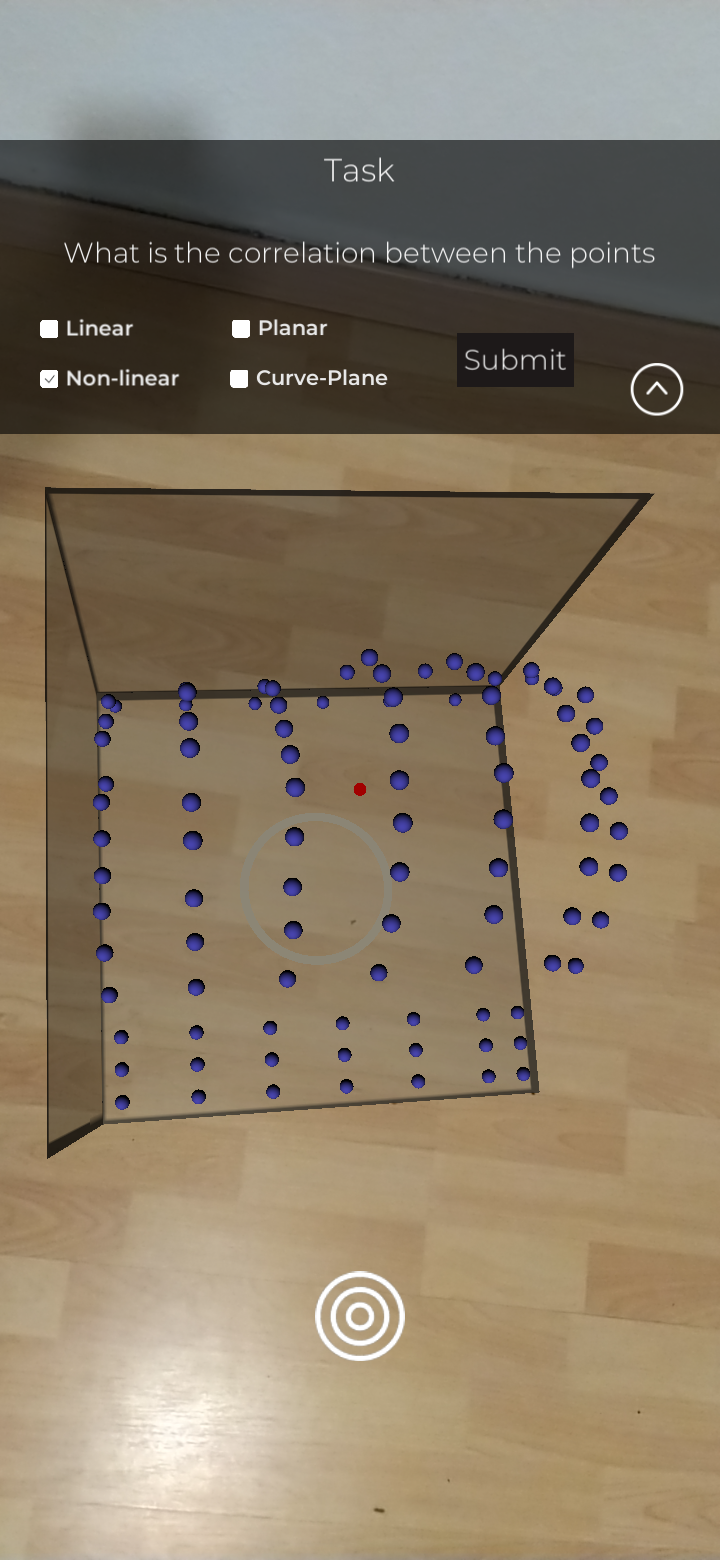
\includegraphics[width=\textwidth, height=2.5in]{correlation_topview.png}
       \subcaption{Top view}
    \end{minipage}
    \caption{Correlation detection task shows random points from front-view, but shows planar correlation from other angles like in top view}
\end{figure}

\subsection{Participants}
The user study would be conducted within the range of 10 to 20 students from the FIN department of Magdeburg University. Users are selected such that they have necessary background knowledge about scatterplot analysis or they have attended one of the courses in Data Mining, Machine Learning or Visual Analytics. Also experts from the Visualization Group at the University of Magdeburg had agreed to participate in the survey.

\section{Hypotheses}
In this project, we propose few hypotheses in the following. It would be interesting to see which of these would be proven right and which of them would be proven wrong by conducting a user study.
\begin{enumerate}
    \item \textit{Participants to perform better in the immersive environment than a non-immersive environment} because of the degree of freedom provided by augmented reality. In the augmented reality environment, the user can freely walk and look around the object as opposed to being stationary in a non-immersive environment.
    \item \textit{Accuracy of detecting the outliers would not differ among the different datasets} because outliers are generally clearly evident since they are far away from the average position of other data points.
    \item \textit{Cluster assignment of data points would be harder as the number of clusters and data points increase} because when there are many clusters and data points, it would be difficult to understand the cluster membership of a data point.
    \item \textit{User interactions to be less in an immersive environment than a non-immersive environment} because of freedom. Consider an example, if the user wants to closely examine a data point, the user might use zooming in a non-immersive scene, whereas, the user could walk towards the point in an immersive scene.
\end{enumerate}

\section{Evaluation}

The user study results could help in making interesting findings as mentioned below.

\begin{enumerate}
    \item[a)] Comparison of participants performance over different datasets in terms of the number of data points.
    \item[b)] Comparison of participants performance between the environment with augmented reality and without augmented reality.
    \item[c)] Immersion levels of participants over the two environments.
    \item[d)] Number of interactions of users in augmented and non-augmented reality environments.
\end{enumerate}
 
\section{Discussion}
In this section, we would have ideally discussed the data collected from the user study. Analyse the graphs from the error rates and time taken to complete each task and summarise the questionnaire filled by the user to check overall preference towards Augmented reality. Unfortunately, at the time of writing this report, the world was hit by an epidemic in the form of COVID-19\cite{Velavan2020}, and the survey was cancelled. Therefore, we tweaked the project to be more of a framework. Nonetheless, we mention some of the observations below which we found while working on the project. 

\subsection{Device Limitations}

A striking limitation is caused by holding the phone for a long time. Even though we are used to, it could lead to fatigue to the user. Further, the screen size of the phone must also be considered, although tiny, it is good enough to analyze a medium-sized dataset but not for a large one.

Another limitation is the performance of the mobile device when the points in the dataset are more than approximately 3500. The rendering starts lagging and manipulation becomes difficult while at the same time, thousands of points are occluded as shown in Fig.

\subsection{Environment Differences}
It has to be noted that both the environments were given the options of zooming and rotating around the only Y-axis. The materials used for the rendering were also the same.

The augmented reality environment showed problems due to differences in light, whereas the non-augmented reality scene showed no effects. In the non-augmented reality, however, the problems were more related to the perception of the data points. This was due to its nature of constant dark background. It is hard to perceive shapes such as the dome-shaped scatterplot in Fig without additional rotations along X and Z axes. However, in the augmented reality environment, the user can perceive such shapes without the need for rotation across different axes because of the degree of freedom to walk around the object.

\begin{figure}[ht]
    \begin{minipage}[b]{0.45\linewidth}
        \centering
        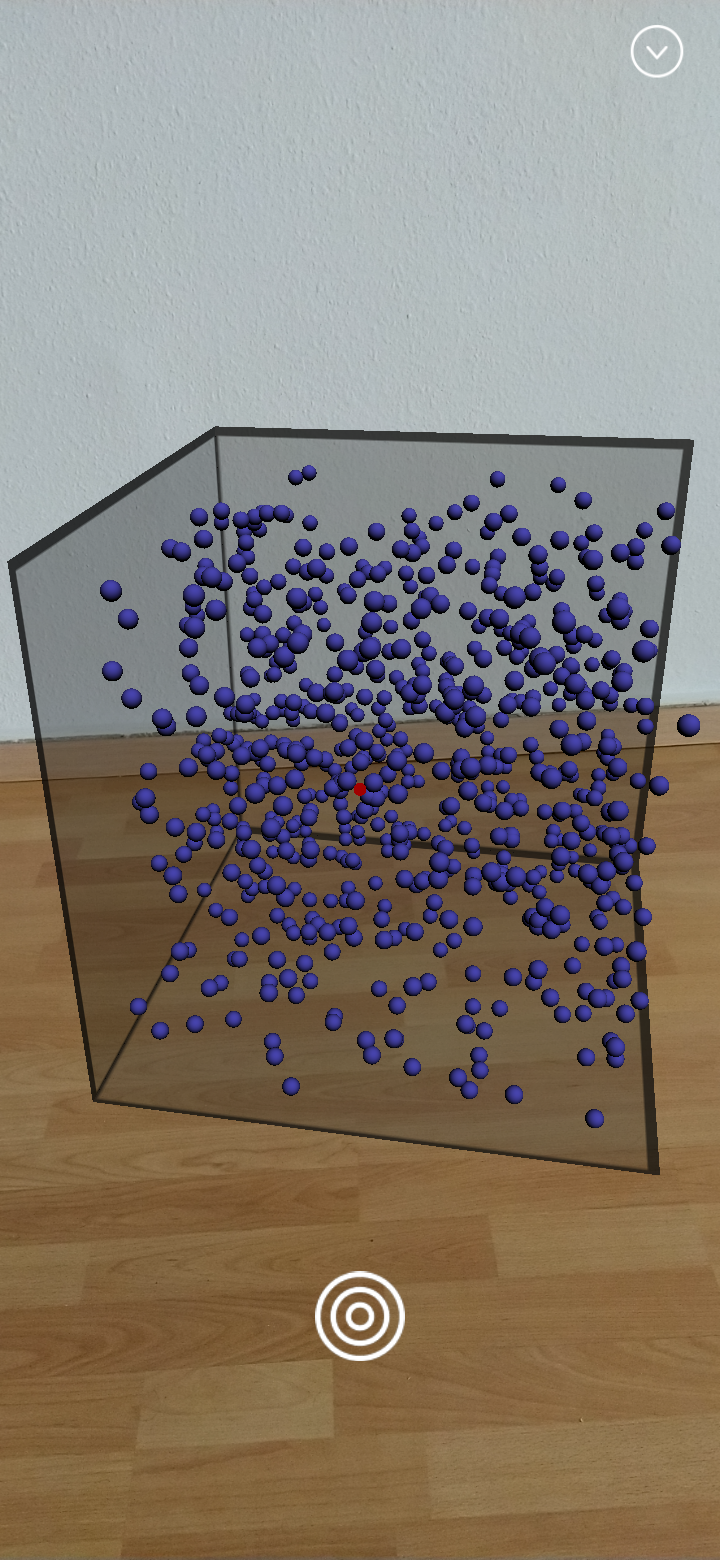
\includegraphics[width=\textwidth, height=2.5in]{700_points.png}
        \subcaption{}
    \end{minipage}
    \hspace{0.5cm}
    \begin{minipage}[b]{0.45\linewidth}
        \centering
        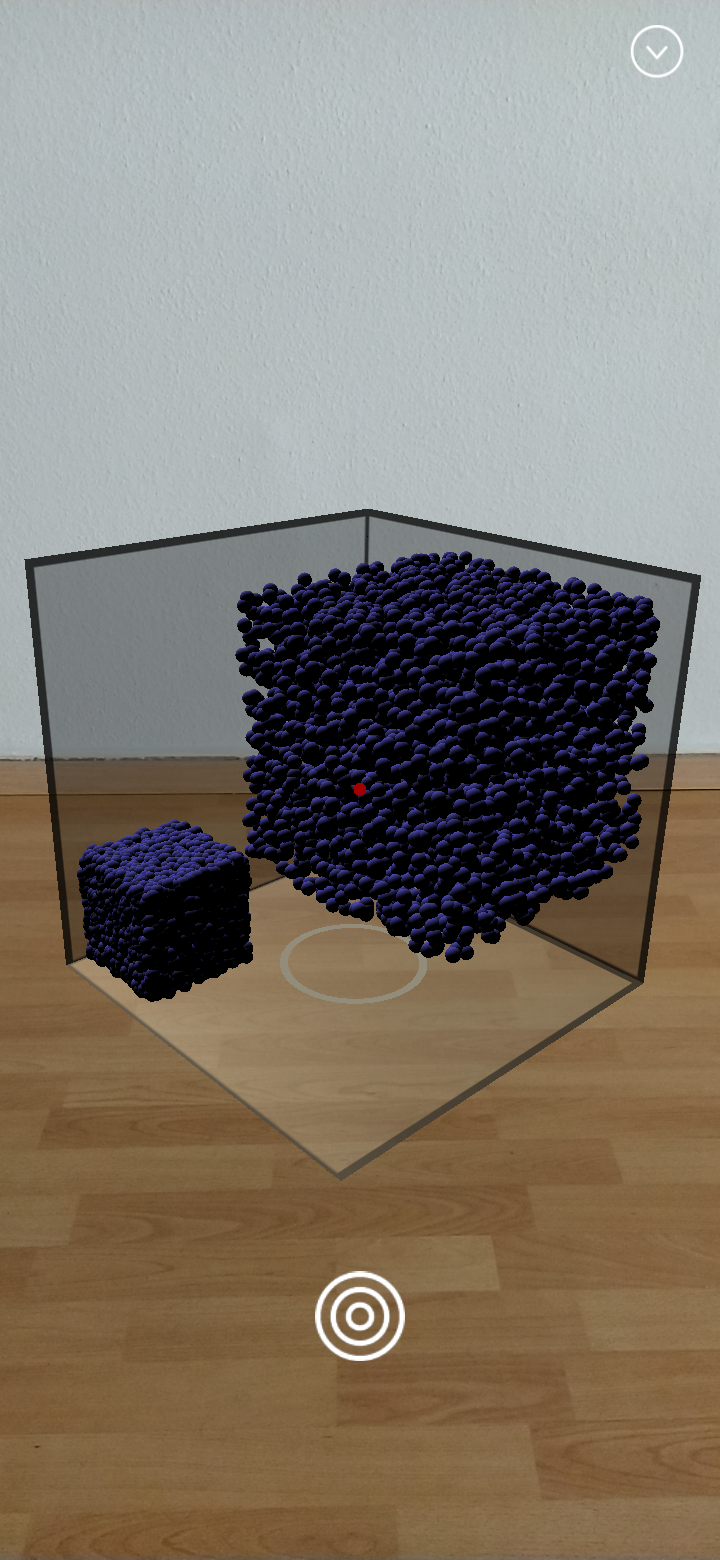
\includegraphics[width=\textwidth, height=2.5in]{20000_points.png}
      \subcaption{}
    \end{minipage}
    \caption{Density of datasets, (a) represents a sparse dataset of 700 points, (b) represents a dense dataset of 20,000 points}
\end{figure}

\section{Conclusions and Future Work}
In this project, we have illustrated a framework for data visualization using the current generation of smartphones. Besides, a controlled user study is proposed on how to measure the effectiveness of the user performance in data analysis using a smartphone. This idea was to show that the current mobile phones have the capabilities to extend their use beyond the typical activities of capturing photos and playing games. We have made use of the latest technology and research conducted in the Immersive Analytics as a baseline for the current work. Even though the smartphones are tiny devices, their current capabilities make them useful for interesting research in Immersive Analytics.

The natural extension to the current work would be to conduct a user study that was discussed in the earlier sections. Based on the results gathered from the user study, further remarks could be made on the effectiveness of data visualization through a mobile phone. To broaden the scope of the current work, another potential comparison between the mobile phone and the HoloLens could be made within an immersive environment. Through this comparison, effects of fatigue, display resolution and semi-transparency could be studied over these two devices. Further, a qualitative evaluation\cite{Preim} could be conducted based on collaborative task solving in this application. This could be analyzed by recording the device screen and the conversation between the two subjects.

\section{Acknowledgements}
We would like to thank the developers of \textit{Unity} and \textit{ARCore} library for providing \textit{easy to work} features. In addition, we would like to also extend our gratitude towards \textit{Plotly} for their datasets which are public and freely available to download. 


%This sounds very very formal 
%The inspiration for this project was derived from 'Visual Analytics',a course offered by the Visualization Group in Otto von Guericke University, Magdeburg. The project was further polished with the help of 'Three-dimensional \& Advanced Interaction', a course offered by Computer-Assisted Surgery Group in Otto von Guericke University, Magdeburg.

\bibliographystyle{abbrv}
%%use following if all content of bibtex file should be shown
%\nocite{*}
\bibliography{template}
\end{document}
